\chapter{Silicon Technology}

The process used in fabricating the chip was the standard 0.6 $\mu$m CMOS process. The CMOS process involves multiple steps that add or remove specific layers of material. To start, a cylindrical (6 inch diameter) ingot of high-purity silicon is created, from which thin (around 500$\mu$m) slices are sawed off called wafers. Chips are square and several milimeters on each side, thus a wafer holds many chips. Due to material and process faults, there are bad areas of the wafer. Chips at these locations do not work, which operational testing is able to determine.

After the wafer is prepared, there were two primary methods used in the CMOS process for this chip: deposition and lithography. Deposition (chemical-vapor deposition, CVD) is a process by which gases or vapors are chemically reacted, leading to the formation of solids on a substrate \cite{microelectronic-circuits}. Common materials for deposition are $\mathrm{SiO_2}$ and $\mathrm{SiNO_3}$. Lithography (also known as photolithography), the second process, is how surface geometry of the various integrated-circuit components is defined. The wafer is coated with a photosensitive layer (called photoresist). A mask will be used to selectively expose the photoresist under ultraviolet light, and the exposed areas will become softened. These areas are then removed using a chemical developer, causing the mask pattern to appear on the wafer.

The simplified fabrication procedure (Fig. \ref{fab-steps}) for the chip began with aluminum being evaporated onto the wafer and patterened using lithography to create probe pads to interface the sensors with the external world, and create contacts and interconnects that carry the sensor current to the probe pads. The chip is deposited with $\mathrm{SiO_2}$ and $\mathrm{SiNO_3}$ to provide insulation between the electrochemical cells and the underlying circuitry. Openings to the probe pads and electrode sites are etched away using lithography. The openings are filled with tungsten to provide contacts between the platinum electrodes and aluminum conductors. The platinum electrodes are fabricated using lithography.

\begin{figure}
\centering
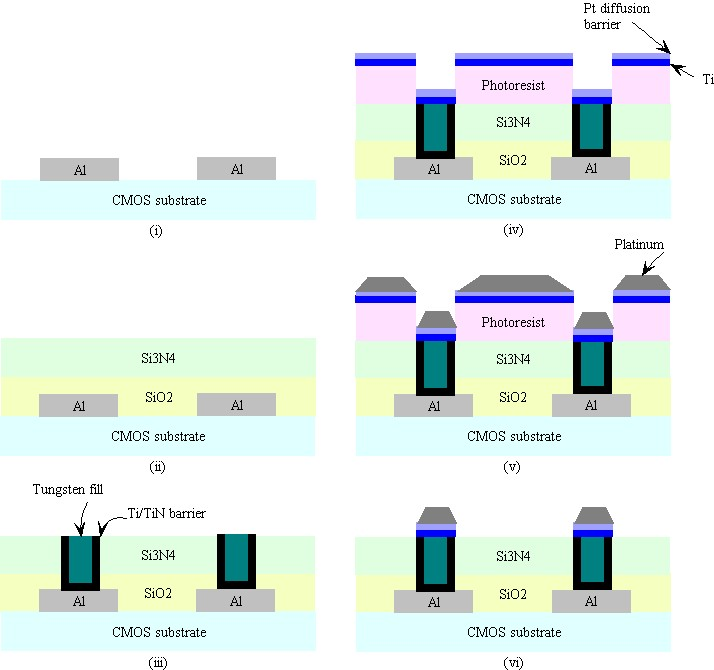
\includegraphics[width=\linewidth]{figures/fabsteps.jpg}
\caption{Fabrication steps and layers.}
\label{fab-steps}
\end{figure}